\documentclass[11pt]{article}

\usepackage[margin=1in]{geometry}
\usepackage[colorlinks=true]{hyperref}
\usepackage{graphicx}
\usepackage{listings}
\usepackage{siunitx}
\usepackage{sidecap}
\usepackage{float}


\begin{document}


ME 331 ThermoFluids

Marcus Hall

Computational Fluid Dynamics Project

\today

\medskip\hrule\medskip

A simulation is considered helpful because of the ability to run thousands of
scenarios that has numerous variations allowing for analysis to be done over a huge
range of data.

\begin{enumerate}
\item Where the pressures are high, the velocities are low. The relations ship
between pressure and velocity is seen in the Bernoulli equation, were as pressure
rises, velocity falls. This means they are in a inverse relationship. They follow
similar curve paths, meaning the isocrones are in similar spots. At the inlet
stagnation point the pressure is $1.47 \si{Pa}$ and the velocity is $0 \si{m/s}$. 

\item 
\begin{figure}[H]
\centering
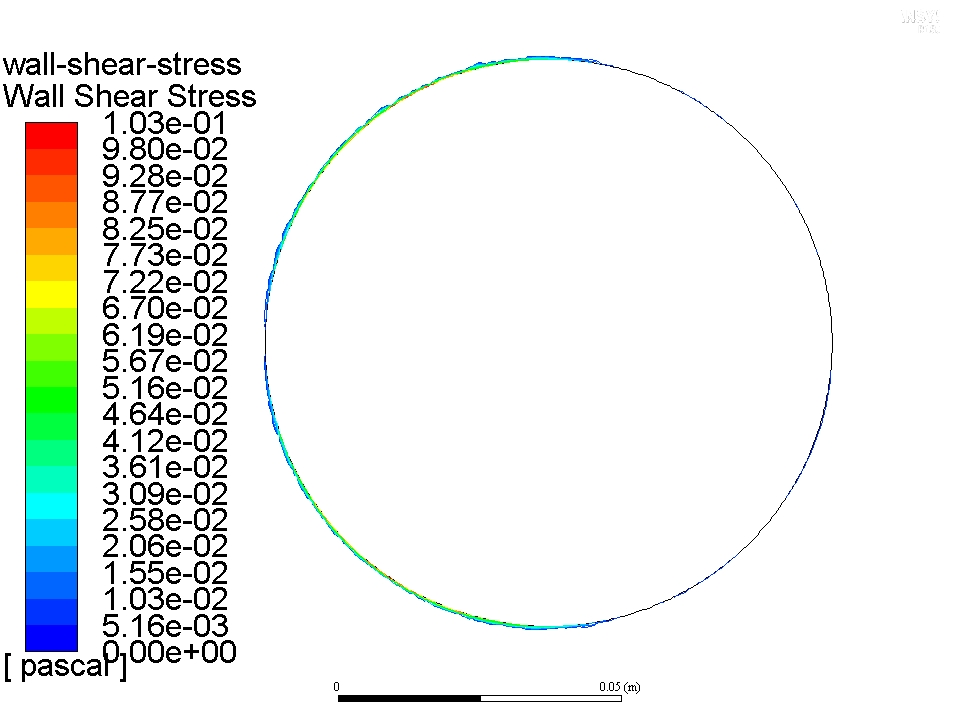
\includegraphics[width=4in]{wall-shear-stress2.jpg}
\caption{Shear Stress around the wall of the Cylinder}
\label{fig:shear}
\end{figure}
As seen in Figure \ref{fig:shear}, shear stress starts right after the
stagnation point and ends about $110^o$ from the front horizonatal. This is seen
where the shear stress drops to zero.


\item In Figure \ref{fig:pressure} the front of the sphere is representative in the
middle of the graph were the static pressure is the greatest. The point at which the flow separates from the wall of the cylinder is at the minimum (there are two representing each side of the cylinder). The vorticities, as representative in Figure \ref{fig:Vmag}, cause the variations in the pressure (or the noise) at those points. The separation occurs at  $0.12$ \& $0.25$.
\begin{figure}[H]
\centering
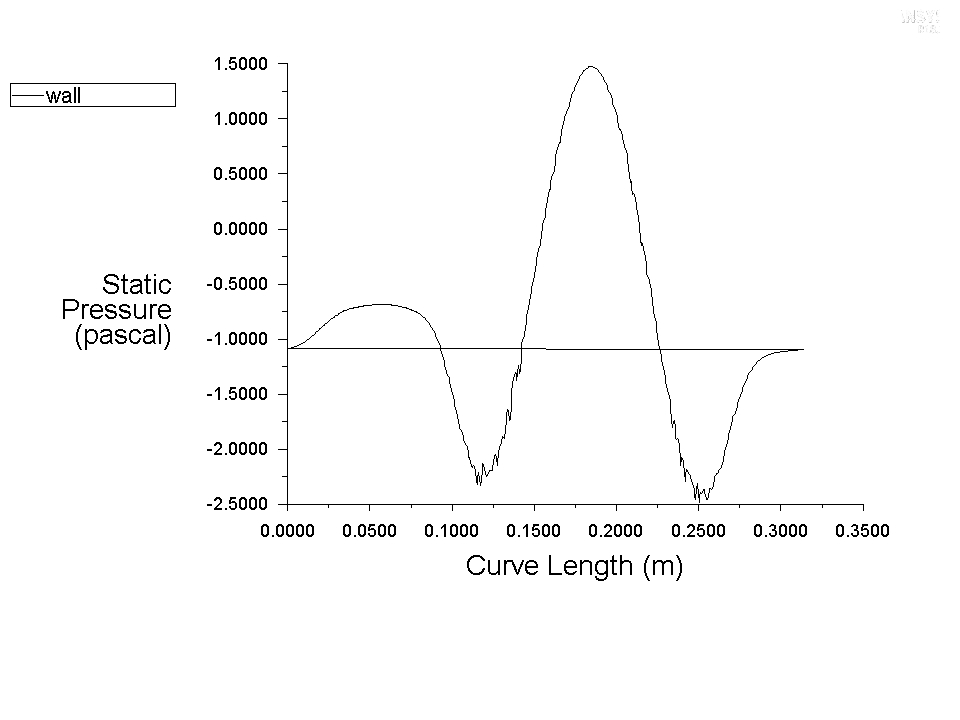
\includegraphics[width=4in]{curve_length_vs_static_pressure.jpg}
\caption{The Static Pressure around the wall of the Cylinder}
\label{fig:pressure}
\end{figure}

\item The computed horizontal force is $F_H = 0.089331025 $. With this information a drag
Coefficient can be calculated using $$C_d = \frac{F_H}{\frac{\pi}{8}\rho V^2 D}$$ Drag Coefficient $C_d = 0.8425169$ 

\item
\begin{figure}[H]
\centering
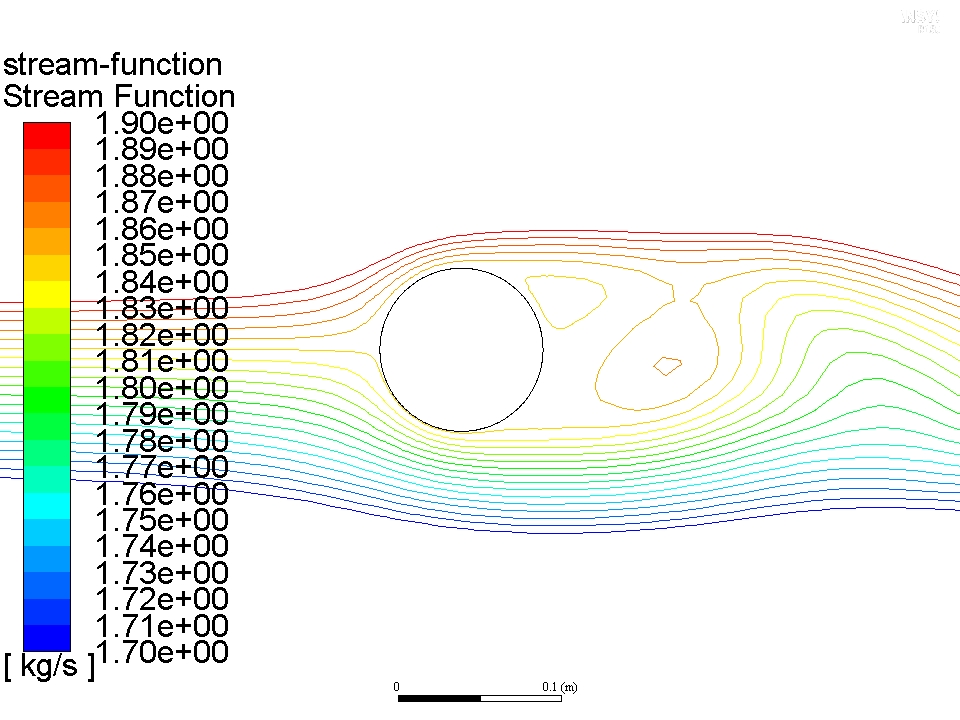
\includegraphics[width=4in]{stream_func.jpg}
\caption{Stream Lines}
\label{fig:Stream}
\end{figure}

\begin{figure}[H]
\centering
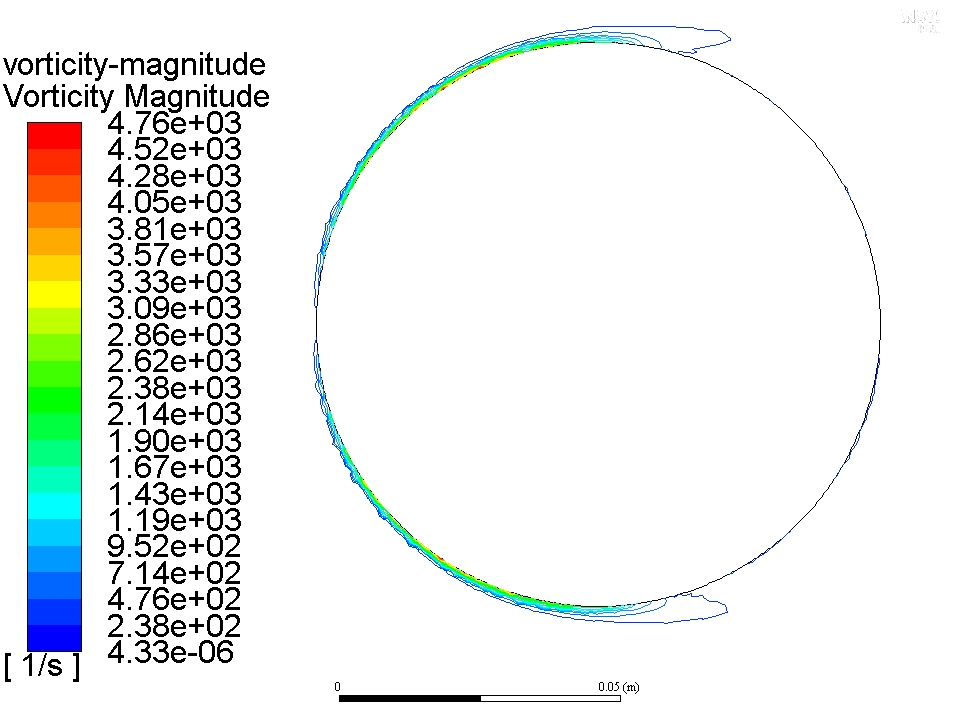
\includegraphics[width=4in]{vorticity.jpg}
\caption{Vorticity Magnitude}
\label{fig:Vmag}
\end{figure}

\item The Karmin frequencies could be calculated along with other things such as turbulent kinetic energy. The graph of turbulent Kinetic energy is Figure \ref{fig:tke}. Or the Strain rate around the surface of cylinder, seen in figure \ref{fig:strainrate}.

\begin{figure}[H]
\centering
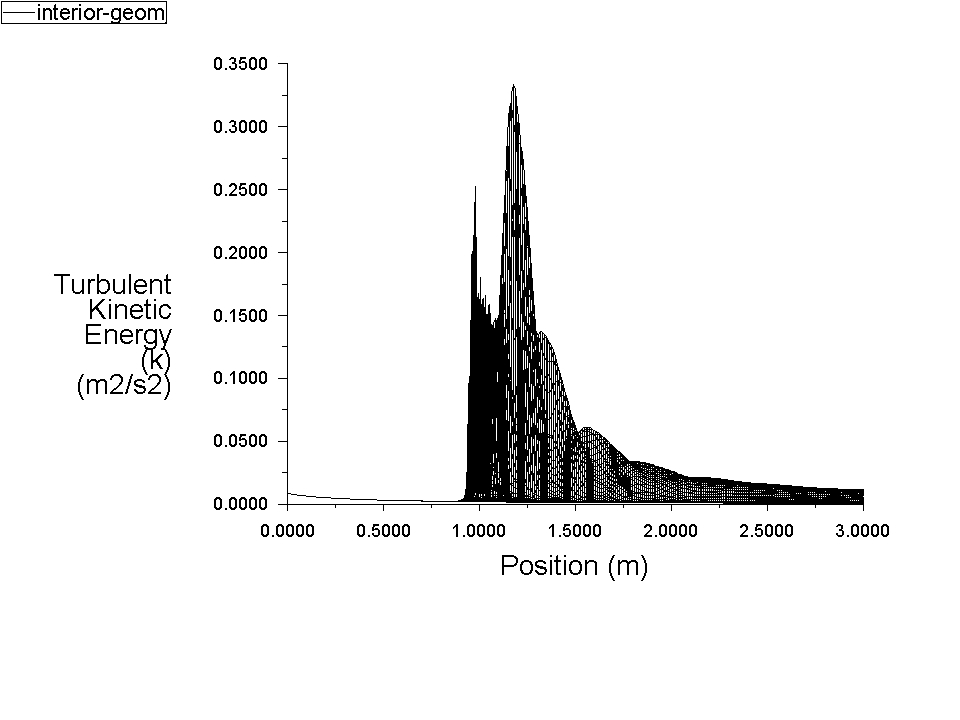
\includegraphics[width=4in]{tke.jpg}
\caption{Turbulent Kinetic Energy}
\label{fig:tke}
\end{figure}

\begin{figure}[H]
\centering
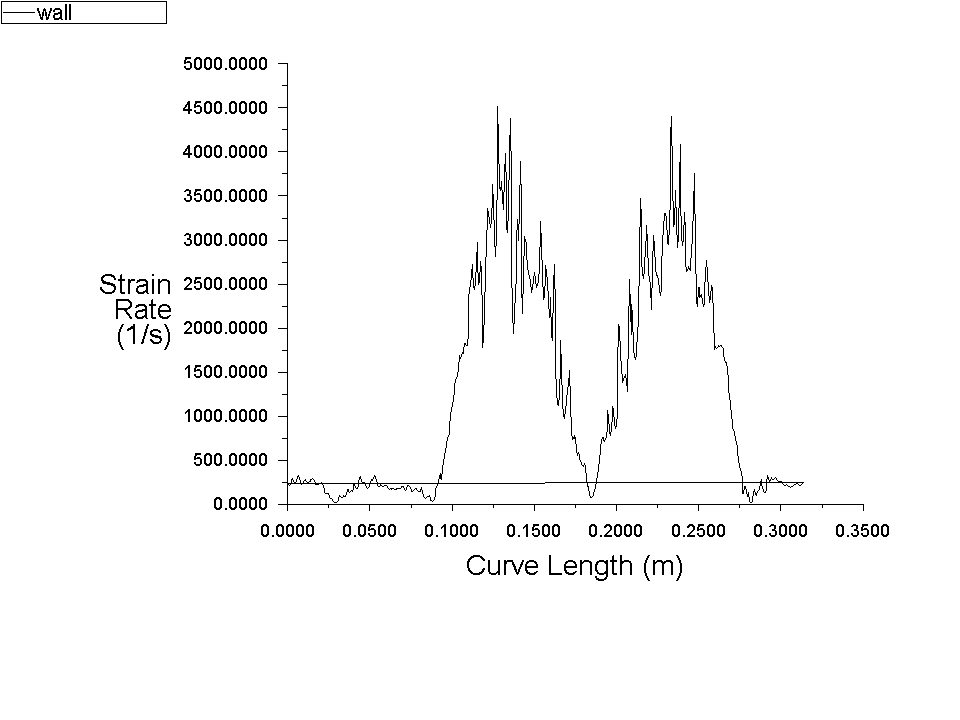
\includegraphics[width=4in]{strainrate.jpg}
\caption{Strain Rate around the surface of the cylinder}
\label{fig:strainrate}
\end{figure}




\end{enumerate}




\end{document}